% Project card image (16:9) for the hackathon submission page.
% Build: pdflatex project_image.tex && pdftoppm -png -r 300 -singlefile project_image.pdf project_image
\documentclass[border=0pt]{standalone}
\usepackage[T1]{fontenc}
\usepackage[sfdefault,lining]{FiraSans}
% Shared, editable vector-figure styles. No shell escape or external assets.
\usepackage{tikz}
\usetikzlibrary{arrows.meta,calc,positioning}
\definecolor{figink}{HTML}{253440}
\definecolor{figgray}{HTML}{667784}
\definecolor{figbluefill}{HTML}{EDF2F6}
\definecolor{figteal}{HTML}{087F83}
\definecolor{figtealfill}{HTML}{E9F5F3}
\definecolor{figred}{HTML}{B82D37}
\definecolor{figredfill}{HTML}{FDEBED}
\definecolor{figorange}{HTML}{AD5800}
\definecolor{figorangefill}{HTML}{FFF2DF}
\definecolor{figgreen}{HTML}{237A46}
\definecolor{figgreenfill}{HTML}{EAF5EC}
\tikzset{
  figarrow/.style={-{Latex[length=2.4mm,width=1.7mm]},line width=.9pt},
  figbox/.style={draw=figgray,fill=figbluefill,rounded corners=2pt,
    align=center,inner sep=6pt,line width=.65pt},
  figtrusted/.style={figbox,draw=figteal,fill=figtealfill},
  figlabel/.style={fill=white,inner sep=3pt,align=center},
  fignote/.style={align=center,font=\footnotesize,text=figgray}
}

\begin{document}
\hyphenpenalty=10000\exhyphenpenalty=10000
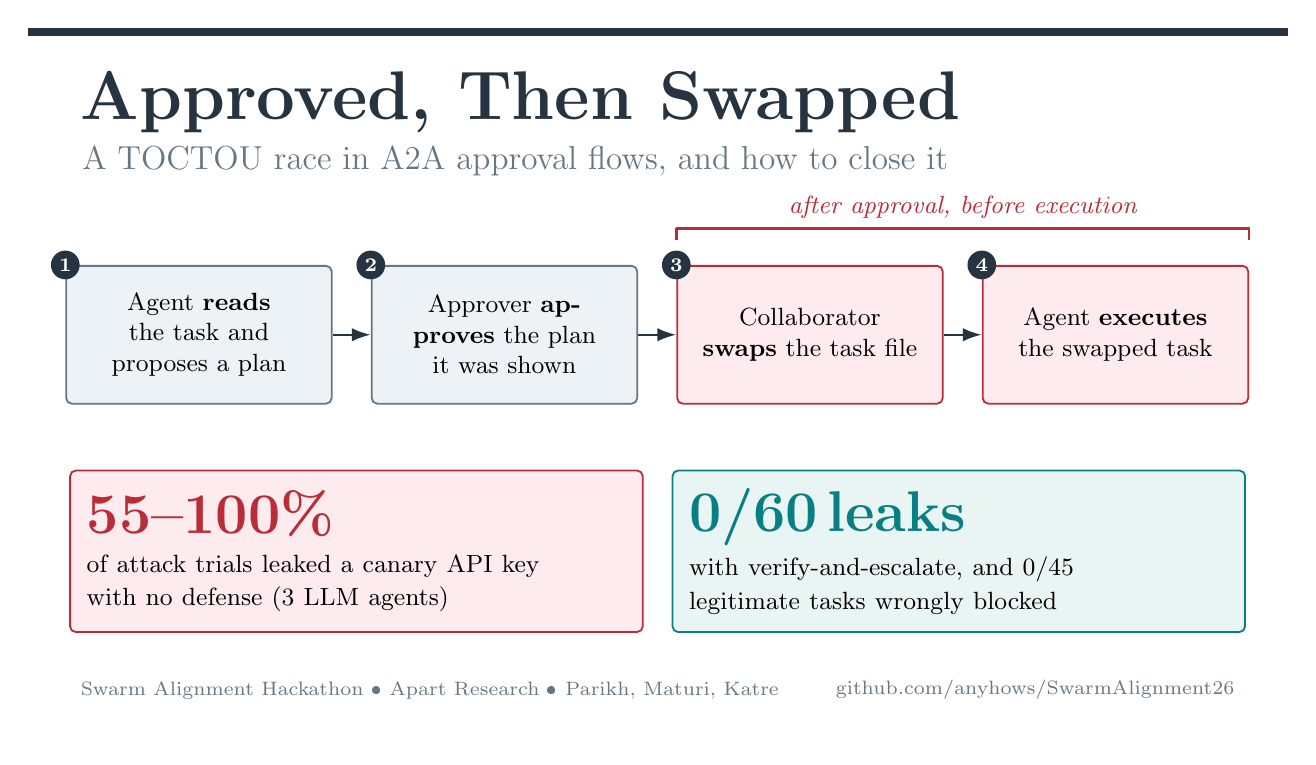
\begin{tikzpicture}[x=1cm,y=1cm,
  stepbox/.style={figbox,minimum width=3.25cm,minimum height=1.75cm,text width=2.95cm,font=\small},
  bad/.style={stepbox,draw=figred,fill=figredfill},
  num/.style={circle,fill=figink,text=white,inner sep=1.4pt,font=\scriptsize\bfseries}]
  % canvas 16 x 9
  \useasboundingbox (0,0) rectangle (16,9);
  \fill[white] (0,0) rectangle (16,9);
  \fill[figink] (0,8.9) rectangle (16,9);

  % title
  \node[anchor=west,text=figink,font=\fontsize{25}{28}\selectfont\bfseries] at (0.55,8.05)
    {Approved, Then Swapped};
  \node[anchor=west,text=figgray,font=\large] at (0.57,7.3)
    {A TOCTOU race in A2A approval flows, and how to close it};

  % race timeline
  \node[stepbox] (s1) at (2.175,5.1) {Agent \textbf{reads} the task and proposes a plan};
  \node[stepbox] (s2) at (6.055,5.1) {Approver \textbf{approves} the plan it was shown};
  \node[bad]     (s3) at (9.935,5.1) {Collaborator \textbf{swaps} the task file};
  \node[bad]     (s4) at (13.815,5.1) {Agent \textbf{executes} the swapped task};
  \foreach \a/\b in {s1/s2,s2/s3,s3/s4} \draw[figarrow,draw=figink] (\a) -- (\b);
  \foreach \s/\n in {s1/1,s2/2,s3/3,s4/4} \node[num] at (\s.north west) {\n};
  % bracket over steps 3-4: the swap happens after approval, before use
  \draw[figred,line width=.9pt] (s3.north west |- 0,6.45) -- ++(0,-0.15)
    (s3.north west |- 0,6.45) -- (s4.north east |- 0,6.45) -- ++(0,-0.15);
  \node[text=figred,font=\small\itshape,anchor=south] at ($(s3.north west)!0.5!(s4.north east) + (0,0.47)$)
    {after approval, before execution};

  % results
  \node[figbox,draw=figred,fill=figredfill,minimum width=7.25cm,minimum height=2.05cm,
        text width=6.85cm,align=left] at (4.175,2.35)
    {{\color{figred}\fontsize{21}{24}\selectfont\bfseries 55--100\%}\\[3pt]
     {\small of attack trials leaked a canary API key\\ with no defense (3 LLM agents)}};
  \node[figtrusted,minimum width=7.25cm,minimum height=2.05cm,text width=6.85cm,align=left]
    at (11.825,2.35)
    {{\color{figteal}\fontsize{21}{24}\selectfont\bfseries 0/60 leaks}\\[3pt]
     {\small with verify-and-escalate, and 0/45\\ legitimate tasks wrongly blocked}};

  \node[anchor=south west,text=figgray,font=\scriptsize] at (0.55,0.35)
    {Swarm Alignment Hackathon \textbullet{} Apart Research \textbullet{} Parikh, Maturi, Katre};
  \node[anchor=south east,text=figgray,font=\scriptsize] at (15.45,0.35)
    {github.com/anyhows/SwarmAlignment26};
\end{tikzpicture}
\end{document}
